\documentclass[aspectratio=169,10pt]{beamer}

\usetheme{Madrid}
\usecolortheme{default}
\setbeamertemplate{navigation symbols}{}
\setbeamertemplate{footline}[frame number]

\usepackage{graphicx}
\usepackage{booktabs}
\usepackage{tabularx}
\usepackage{colortbl}
\usepackage{movie15}
\usepackage{tikz}
\usepackage{amsmath}
\usetikzlibrary{positioning,shapes.symbols}

\graphicspath{{images/}}

\definecolor{HHUBlue}{RGB}{0,61,124}
\definecolor{HHULight}{RGB}{235,242,249}
\definecolor{LTGreen}{RGB}{52,160,119}
\definecolor{LTLight}{RGB}{232,245,238}
\definecolor{WinRateExcellent}{rgb}{0.86,0.93,0.86}
\definecolor{WinRateGood}{rgb}{0.91,0.96,0.91}
\definecolor{WinRateMedium}{rgb}{0.97,0.98,0.90}
\definecolor{WinRateLow}{rgb}{0.99,0.95,0.88}
\definecolor{WinRateWeak}{rgb}{0.98,0.90,0.90}
\definecolor{WinRateExcellentMark}{RGB}{57,156,102}
\definecolor{WinRateGoodMark}{RGB}{141,190,87}
\definecolor{WinRateMediumMark}{RGB}{231,202,77}
\definecolor{WinRateLowMark}{RGB}{230,140,59}
\definecolor{WinRateWeakMark}{RGB}{211,79,73}
\newcommand{\TrainingPipelineCardWidth}{0.98\linewidth}
\newcommand{\TrainingPipelineBoxHeight}{1.35cm}
\newcommand{\TrainingPipelineCard}[4]{%
    \begingroup
    \setbeamercolor{pipeline title}{bg=#1,fg=white}%
    \setbeamercolor{pipeline body}{bg=#2,fg=black}%
    \centering
    \begin{beamerboxesrounded}[upper=pipeline title,lower=pipeline body,shadow=true,width=\TrainingPipelineCardWidth]{#3}
        \parbox[t][\TrainingPipelineBoxHeight][t]{0.94\linewidth}{%
            \raggedright\small #4%
        }
    \end{beamerboxesrounded}
    \endgroup
}
\newcommand{\SizedTrainingPipelineCard}[6]{%
    \begingroup
    \renewcommand{\TrainingPipelineCardWidth}{#1}%
    \renewcommand{\TrainingPipelineBoxHeight}{#2}%
    \TrainingPipelineCard{#3}{#4}{#5}{#6}%
    \endgroup
}

\newcommand{\WinRateCellText}[2]{%
    \begingroup
    \ifdim #1pt > 94.9pt
        \cellcolor{WinRateExcellent}#2%
    \else
        \ifdim #1pt > 84.9pt
            \cellcolor{WinRateGood}#2%
        \else
            \ifdim #1pt > 69.9pt
                \cellcolor{WinRateMedium}#2%
            \else
                \ifdim #1pt > 49.9pt
                    \cellcolor{WinRateLow}#2%
                \else
                    \cellcolor{WinRateWeak}#2%
                \fi
            \fi
        \fi
    \fi
    \endgroup
}
\newcommand{\WinRateCell}[1]{\WinRateCellText{#1}{#1}}
\newcommand{\BestWinRateCell}[1]{\WinRateCellText{#1}{\textbf{#1}}}
\newcommand{\WinRateMarkWidth}{3.8em}
\newcommand{\WinRateMarkHeight}{2.45ex}
\newcommand<>{\WinRateValueMark}[2]{%
    \makebox[\WinRateMarkWidth][c]{%
        \alt#3{%
            \tikz[baseline=(winratemark.base)]{%
                \node[
                    draw=#1!65!black,
                    fill=#1,
                    fill opacity=0.45,
                    text opacity=1,
                    line width=0.8pt,
                    rounded corners=1pt,
                    minimum width=\WinRateMarkWidth,
                    minimum height=\WinRateMarkHeight,
                    inner sep=0pt,
                    text height=1.55ex,
                    text depth=0.45ex,
                    outer sep=0pt
                ] (winratemark) {\strut #2};%
            }%
        }{\strut #2}%
    }%
}
\newcommand<>{\MarkedWinRateCellText}[2]{%
    \begingroup
    \ifdim #1pt > 94.9pt
        \cellcolor{WinRateExcellent}\WinRateValueMark#3{WinRateExcellentMark}{#2}%
    \else
        \ifdim #1pt > 84.9pt
            \cellcolor{WinRateGood}\WinRateValueMark#3{WinRateGoodMark}{#2}%
        \else
            \ifdim #1pt > 69.9pt
                \cellcolor{WinRateMedium}\WinRateValueMark#3{WinRateMediumMark}{#2}%
            \else
                \ifdim #1pt > 49.9pt
                    \cellcolor{WinRateLow}\WinRateValueMark#3{WinRateLowMark}{#2}%
                \else
                    \cellcolor{WinRateWeak}\WinRateValueMark#3{WinRateWeakMark}{#2}%
                \fi
            \fi
        \fi
    \fi
    \endgroup
}
\newcommand{\LossRateCellText}[2]{%
    \begingroup
    \ifdim #1pt < 2.1pt
        \cellcolor[rgb]{0.86,0.93,0.86}#2%
    \else
        \ifdim #1pt < 8.1pt
            \cellcolor[rgb]{0.91,0.96,0.91}#2%
        \else
            \ifdim #1pt < 18.1pt
                \cellcolor[rgb]{0.99,0.95,0.88}#2%
            \else
                \cellcolor[rgb]{0.98,0.90,0.90}#2%
            \fi
        \fi
    \fi
    \endgroup
}
\newcommand{\LossRateCell}[1]{\LossRateCellText{#1}{#1}}
\newcommand{\BestLossRateCell}[1]{\LossRateCellText{#1}{\textbf{#1}}}
\newcommand<>{\ResultMark}[1]{%
    \alt#2{%
        \tikz[baseline=(resultmark.base)]{%
            \node[
                draw=LTGreen,
                fill=LTGreen!18,
                line width=0.7pt,
                rounded corners=1.5pt,
                inner xsep=1.8pt,
                inner ysep=0.9pt,
                text height=1.55ex,
                text depth=0.45ex,
                outer sep=0pt
            ] (resultmark) {\strut #1};%
        }%
    }{#1}%
}
\newcommand<>{\WarningMark}[1]{%
    \alt#2{%
        \tikz[baseline=(warningmark.base)]{%
            \node[
                draw=orange!85!black,
                fill=orange!18,
                line width=0.7pt,
                rounded corners=1.5pt,
                inner xsep=1.8pt,
                inner ysep=0.9pt,
                text height=1.55ex,
                text depth=0.45ex,
                outer sep=0pt
            ] (warningmark) {\strut #1};%
        }%
    }{#1}%
}
\newcommand<>{\MarkedOpponent}[1]{\ResultMark#2{#1}}
\newcommand<>{\MarkedWinRateCell}[1]{\MarkedWinRateCellText#2{#1}{#1}}
\newcommand<>{\MarkedBestWinRateCell}[1]{\MarkedWinRateCellText#2{#1}{\textbf{#1}}}
\newcommand<>{\WarningWinRateCell}[1]{\MarkedWinRateCellText#2{#1}{#1}}
\newcommand<>{\WarningBestWinRateCell}[1]{\MarkedWinRateCellText#2{#1}{\textbf{#1}}}

\setbeamercolor{structure}{fg=HHUBlue}
\setbeamercolor{palette primary}{bg=HHUBlue,fg=white}
\setbeamercolor{palette secondary}{bg=HHUBlue,fg=white}
\setbeamercolor{palette tertiary}{bg=HHUBlue,fg=white}
\setbeamercolor{title}{fg=white,bg=HHUBlue}
\setbeamercolor{subtitle}{fg=white}
\setbeamercolor{frametitle}{fg=HHUBlue,bg=HHULight}
\setbeamercolor{block title}{bg=HHUBlue,fg=white}
\setbeamercolor{block body}{bg=HHULight,fg=black}

\title[League Training in MicroRTS]{Implementation and evaluation of the reinforcement learning methods\\Self-Play and League Training in the MicroRTS environment}
\author{Niklas Glaser}
\institute{Heinrich-Heine-Universit\"at D\"usseldorf}
\date{April 2026}

\begin{document}

\begin{frame}
    \titlepage
    \vspace{-1.5em}
    \begin{center}
        
\includegraphics[width=0.16\linewidth]{hhu_logo.png}
    \end{center}
\end{frame}

% \begin{frame}{Overview}
%     \tableofcontents
% \end{frame}

\section{Motivation}



\begin{frame}{Goals and Research Question}
    \small
    \begin{block}{Goal}
        \begin{itemize}
            \item improve the Base Agent with League Training (LT)
            \item training against a more diverse set of opponents
            \item focus on robustness and generalization
        \end{itemize}
    \end{block}
    \begin{block}{Base Agent}
        \begin{itemize}
            \item combination of Behavioral Cloning (BC) and Proximal Policy Optimization (PPO)
            \item strong baseline, but weaknesses against several opponents
        \end{itemize}
    \end{block}
    \begin{alertblock}{Research Question}
        \begin{itemize}
            \item How much does LT with PPO improve robustness and generalization of the BC/PPO-pretrained agent?
            \item How strongly does this depend on the diversity of initial agents and BC experts?
        \end{itemize}
    \end{alertblock}
\end{frame}


\begin{frame}{Setting}
    \small
    \begin{columns}[T]
        \begin{column}{0.52\textwidth}
            \begin{block}{MicroRTS}
                \begin{itemize}
                    \item simplified RTS environment for RL research
                    \item still contains resource management, unit production and combat
                    \item supports controlled and repeatable experiments
                \end{itemize}
            \end{block}
            \begin{block}{Main RL challenges}
                \begin{itemize}
                    \item large combinatorial action space
                    \item simultaneous decisions
                    \item delayed and sparse rewards
                    \item robustness against diverse opponents
                \end{itemize}
            \end{block}
            \vspace{0.4em}
            \begin{center}
                \href{run:images/MicroRTS_example.mp4}{\beamergotobutton{Open MicroRTS Example Video}}
            \end{center}
        \end{column}
        \begin{column}{0.45\textwidth}
            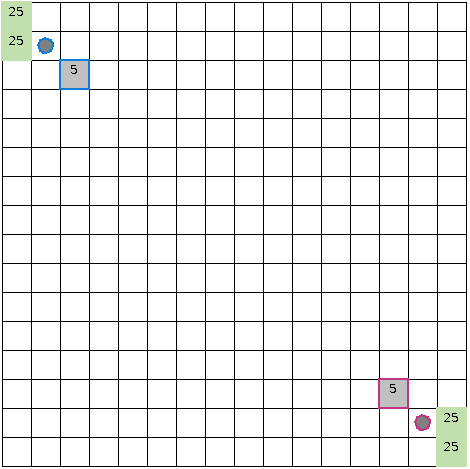
\includegraphics[width=0.94\linewidth]{initial_pos_basesWorkers16x16A.png}
        \end{column}
    \end{columns}
\end{frame}


\section{Approach}

\begin{frame}{Training Pipeline}
    \centering
    \begin{tikzpicture}[
        node distance=0.16cm,
        stage/.style={
            draw=HHUBlue,
            fill=HHULight,
            text=HHUBlue,
            signal,
            signal from=west,
            signal to=east,
            line width=0.8pt,
            minimum height=0.92cm,
            inner xsep=4pt,
            align=center,
            font=\bfseries\footnotesize
        },
        focusstage/.style={
            stage,
            draw=LTGreen,
            fill=LTGreen,
            text=white
        }
    ]
        \node[stage, minimum width=2.00cm] (bc) {BC};
        \node[stage, minimum width=2.00cm, right=of bc] (bcft) {BC-FT};
        \node[stage, minimum width=2.00cm, right=of bcft] (ppo) {PPO};
        \node[focusstage, minimum width=2.00cm, right=of ppo] (lt) {LT};
        \node[stage, minimum width=2.00cm, right=of lt] (ft) {PPO fine-tuning};
    \end{tikzpicture}

    \vspace{0.9em}

    \noindent
    \begin{minipage}[t]{0.49\textwidth}
        \TrainingPipelineCard{HHUBlue}{HHULight}{BC and BC-FT}{
            \begin{itemize}
                \item imitate experts
                \item BC-FT: only winning replays
            \end{itemize}
            }
    \end{minipage}\hfill
    \begin{minipage}[t]{0.49\textwidth}
        \TrainingPipelineCard{HHUBlue}{HHULight}{PPO}{
            \begin{itemize}
                \item iteratively update policy
                \item refine the policy through exploration
            \end{itemize}
            }
    \end{minipage}

    \vspace{0.2em}

    \noindent
    \begin{minipage}[t]{0.49\textwidth}
        \TrainingPipelineCard{LTGreen}{LTLight}{LT}{
            \begin{itemize}
                \item train against an evolving opponent population
                \item add exploiters
            \end{itemize}
        }
    \end{minipage}\hfill
    \begin{minipage}[t]{0.49\textwidth}
        \TrainingPipelineCard{HHUBlue}{HHULight}{PPO fine-tuning}{
            \begin{itemize}
                \item repair the main remaining weakness after LT
                \item add WorkerRushAI as opponent
            \end{itemize}
            }
    \end{minipage}
\end{frame}

\begin{frame}{From SP to LT}
    \centering
    \begin{tikzpicture}[
        node distance=1.45cm,
        method/.style={
            draw=HHUBlue,
            fill=HHULight,
            text=HHUBlue,
            rounded corners=2pt,
            line width=0.8pt,
            minimum width=1.65cm,
            minimum height=0.72cm,
            inner xsep=6pt,
            align=center,
            font=\bfseries\footnotesize
        },
        focusmethod/.style={
            method,
            draw=LTGreen,
            fill=LTLight,
            text=LTGreen
        },
        addlabel/.style={
            font=\scriptsize,
            align=center,
            text=HHUBlue
        }
    ]
        \node[addlabel, text=black!65] at (3.3,0.85) {};
        \node[method] (sp) {SP};
        \node[method, right=of sp] (fsp) {FSP};
        \node[method, right=of fsp] (pfsp) {PFSP};
        \node[focusmethod, right=of pfsp] (lt) {LT};

        \draw[->, line width=0.8pt, HHUBlue] (sp.east) -- node[addlabel, above] {+ snapshots} (fsp.west);
        \draw[->, line width=0.8pt, HHUBlue] (fsp.east) -- node[addlabel, above] {+ win-rate\\sampling} (pfsp.west);
        \draw[->, line width=0.8pt, LTGreen] (pfsp.east) -- node[addlabel, above, text=LTGreen] {SP + PFSP and\\exploiters} (lt.west);
    \end{tikzpicture}

    \vspace{0.45em}

    {
    \renewcommand{\TrainingPipelineBoxHeight}{3.85cm}
    \begin{columns}[T,onlytextwidth]
        \begin{column}{0.40\textwidth}
            \TrainingPipelineCard{HHUBlue}{HHULight}{cyclical learning of SP}{
                \begin{center}
                    \begin{tikzpicture}[
                        scale=0.9,
                        every node/.style={font=\small},
                        learnarrow/.style={->, line width=1pt, HHUBlue, shorten <=4pt, shorten >=4pt},
                        goodagainst/.style={->, line width=1pt, red!75!black}
                    ]
                        \node[circle, draw=HHUBlue, line width=1pt, minimum size=0.7cm, inner sep=0pt] (a) at (0,1.2) {\textbf{A}};
                        \node[circle, draw=HHUBlue, line width=1pt, minimum size=0.7cm, inner sep=0pt] (b) at (-1.0,-0.45) {\textbf{B}};
                        \node[circle, draw=HHUBlue, line width=1pt, minimum size=0.7cm, inner sep=0pt] (c) at (1.0,-0.45) {\textbf{C}};
                        \draw[learnarrow] (a) -- (b);
                        \draw[learnarrow] (b) -- (c);
                        \draw[learnarrow] (c) -- (a);
                        \draw[goodagainst] (b) to[out=120,in=180,looseness=1.35] (a);
                        \draw[goodagainst] (a) to[out=0,in=60,looseness=1.35] (c);
                        \draw[goodagainst] (c) .. controls (0.55,-1.02) and (-0.55,-1.02) .. (b);
                        \node[font=\scriptsize, text=black!70, align=center, text width=3.9cm] at (0,-1.68) {%
                            {\color{HHUBlue}Blue arrows}: learning direction\\
                            {\color{red!75!black}Red arrows}: policies the current policy performs well against%
                        };
                    \end{tikzpicture}
                \end{center}
            }
        \end{column}
        \begin{column}{0.58\textwidth}
            \TrainingPipelineCard{LTGreen}{LTLight}{Why LT helps}{
                \begin{itemize}
                    \setlength{\itemsep}{0.22em}
                    \item improves stability by identifying and exploiting weaknesses
                    \item creates diverse set of opponents without the main agent having to find them through exploration
                \end{itemize}
            }
        \end{column}
    \end{columns}
    }
\end{frame}

\begin{frame}{LT Design}
    \noindent
    \begin{minipage}[t]{0.49\textwidth}
        \TrainingPipelineCard{HHUBlue}{HHULight}{Main Agent (MA)}{
            \begin{itemize}
                \item primary policy
                \item resulting agent
            \end{itemize}
            }
    \end{minipage}\hfill
    \begin{minipage}[t]{0.49\textwidth}
        \TrainingPipelineCard{HHUBlue}{HHULight}{Historical Agents (HA)}{
            \begin{itemize}
                \item frozen checkpoints kept in the opponent pool
                \item created by all other league agent types
            \end{itemize}
            }
    \end{minipage}

    \vspace{0.2em}

    \noindent
    \begin{minipage}[t]{0.49\textwidth}
        \TrainingPipelineCard{HHUBlue}{HHULight}{Main Exploiters (ME)}{
            \begin{itemize}
                \item exploit weaknesses of the MA
                \item reset when checkpointed
            \end{itemize}
        }
    \end{minipage}\hfill
    \begin{minipage}[t]{0.49\textwidth}
        \TrainingPipelineCard{HHUBlue}{HHULight}{League Exploiters (LE)}{
            \begin{itemize}
                \item exploit broader weaknesses across the league
                \item can reset when checkpointed
            \end{itemize}
            }
    \end{minipage}
\end{frame}

\begin{frame}{LT MA Matchmaking}
    \begin{columns}[T]
        \begin{column}{0.52\textwidth}
            \begin{center}
                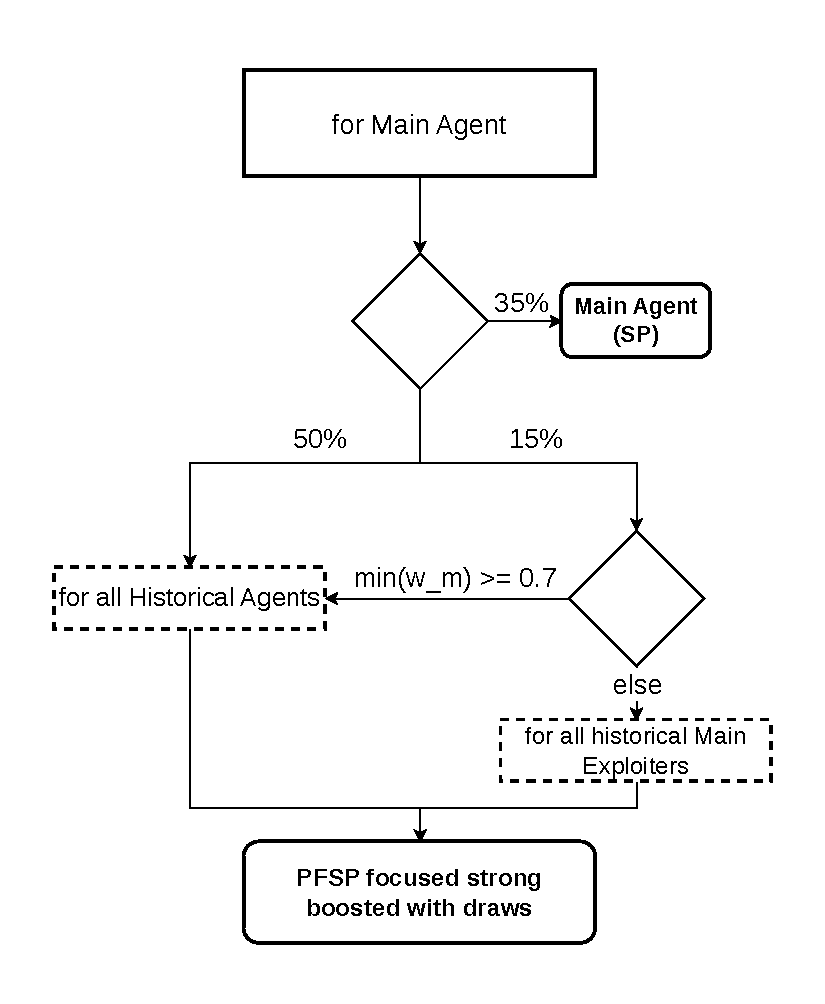
\includegraphics[width=\linewidth,height=0.74\textheight,keepaspectratio]{diagram_with_obs_only_MA.pdf}
            \end{center}
        \end{column}
        \begin{column}{0.45\textwidth}
            \begin{center}
                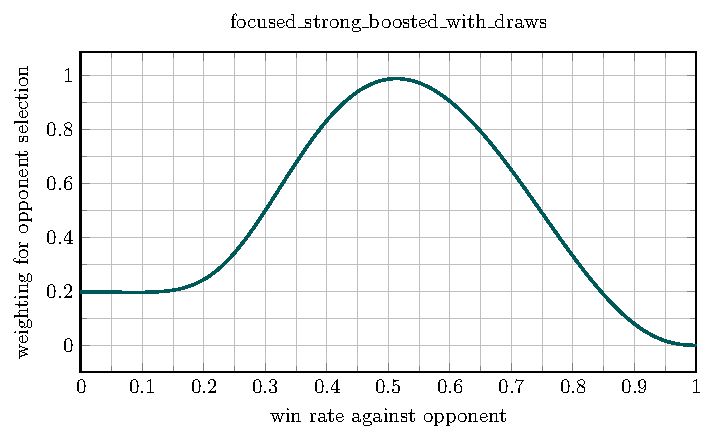
\includegraphics[width=\linewidth,height=0.42\textheight,keepaspectratio]{focused_strong_boosted_with_draws.pdf}
            \end{center}
            \small
            \begin{itemize}
                \item 35\% self-play
                \item 50\% PFSP over HAs
                \item 15\% PFSP over HMEs if win rate is low
                \item PFSP prioritizes unresolved matchups
            \end{itemize}
        \end{column}
    \end{columns}
\end{frame}

\begin{frame}{Bot Environments}
    \begin{columns}[T]
        \begin{column}{0.52\textwidth}
            \SizedTrainingPipelineCard{\linewidth}{2.05cm}{HHUBlue}{HHULight}{Bot environments}{%
                \begin{itemize}
                    \item additional dynamic bot environments (CoacAI and Mayari)% to stabilize the early LT phase
                    \item scripted bots: CoacAI, Mayari, WorkerRushAI, PassiveAI, LightRushAI, RandomAI and RandomBiasedAI
                    \item MCTS based bots: Rojo, MixedBot, Izanagi, Tiamat, Droplet, GuidedRojoA3N and NaiveMCTS
                \end{itemize}
            }
        \end{column}
        \begin{column}{0.45\textwidth}
            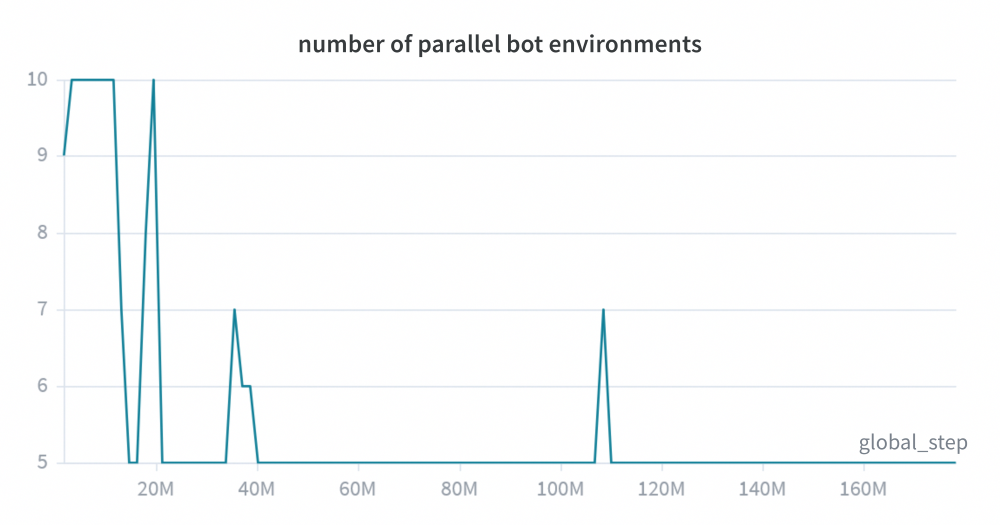
\includegraphics[width=\linewidth]{num_parallel_bot_envs.png}
        \end{column}
    \end{columns}
\end{frame}

\begin{frame}{Observation Adjustment for SP}
    \SizedTrainingPipelineCard{0.78\linewidth}{1.45cm}{HHUBlue}{HHULight}{Observation adjustment}{%
        \begin{itemize}
            \item Base Agent only trained as Player 1
            \item flip Player-2 GridNet observations
            \item flip masks and action directions
        \end{itemize}
    }
    \vspace{0.1em}
    {\centering
        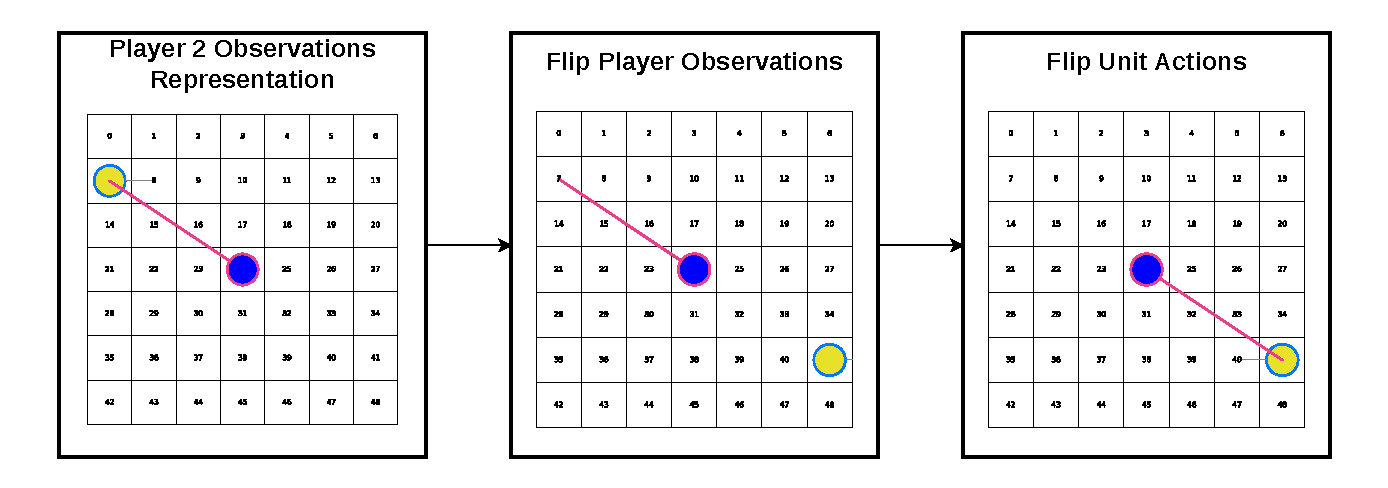
\includegraphics[width=\linewidth,height=0.53\textheight,keepaspectratio]{adjust_obs_präsentation.pdf}
        \par
    }
\end{frame}

\begin{frame}{Implementation Changes}
    \centering
    \SizedTrainingPipelineCard{0.82\linewidth}{1.55cm}{HHUBlue}{HHULight}{Key changes}{%
        \begin{itemize}
            % only Player 2 rotation
            \item delta score reward: denser signal in sparse-reward games
            \item annealed entropy coefficient: more exploration early, less later
            \item new initial agents: new start points for exploiters
        \end{itemize}
    }
\end{frame}


\section{Experiments}

\begin{frame}{Experiment Setup}
    \begin{columns}[T]
        \begin{column}{0.52\textwidth}
            \SizedTrainingPipelineCard{\linewidth}{3.55cm}{HHUBlue}{HHULight}{Setup}{%
                \begin{itemize}
                    \item 1 map: \texttt{basesWorkers16x16A}
                    \item 1 MA, 4 ME, 1 LE
                    \item for each 25 environments
                    \item 5 to 10 dynamic bot environments
                    \item \(\sim\)130M LT steps, \(\sim\)100 h
                    \item max: 160 parallel environments
                    \item eval: at least 100 games vs 12 opponents
                \end{itemize}
            }
        \end{column}
        \begin{column}{0.45\textwidth}
            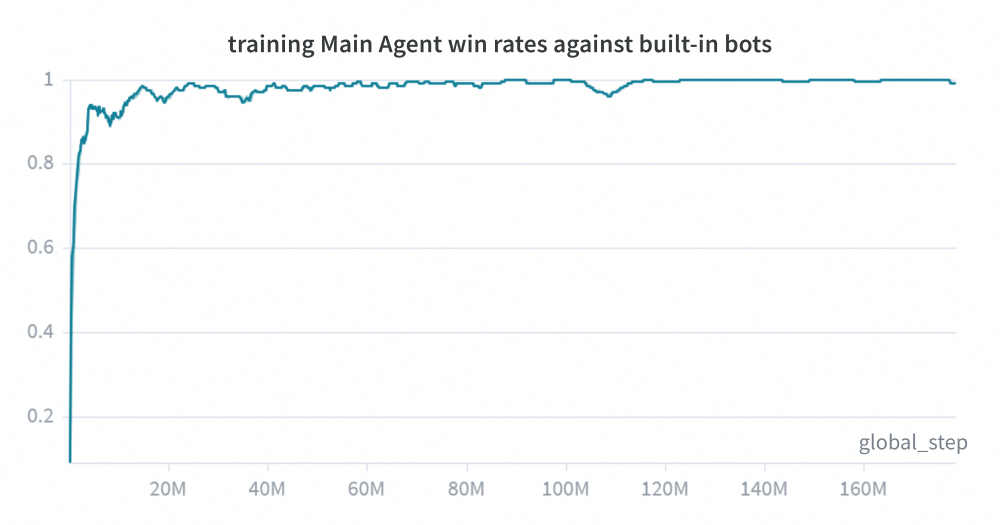
\includegraphics[width=\linewidth]{bot_win_rates_no_draw.png}
        \end{column}
    \end{columns}
\end{frame}

\section{Results}

\begin{frame}{Main Quantitative Result}
    \begin{columns}[T]
        \begin{column}{0.68\textwidth}
            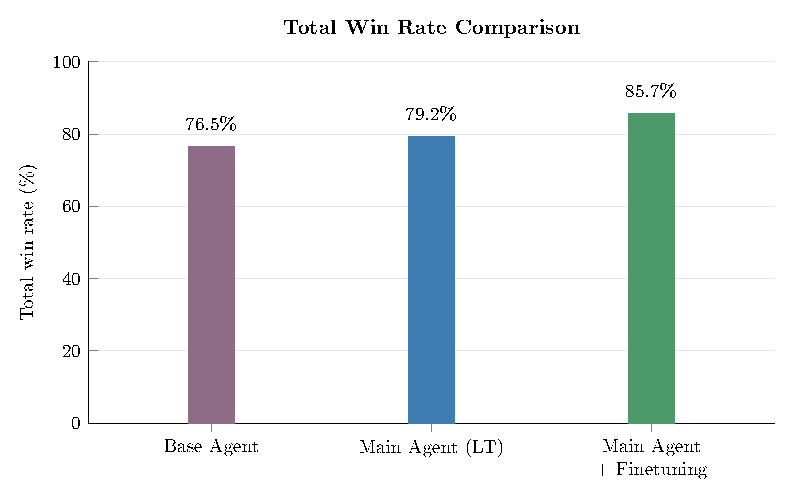
\includegraphics[width=\linewidth]{abstract_total_winrate_comparison.pdf}
        \end{column}
        \begin{column}{0.28\textwidth}
            \SizedTrainingPipelineCard{\linewidth}{2.25cm}{HHUBlue}{HHULight}{Loss rate}{%
                \begin{itemize}
                    \item loss rate: \textbf{7.7\%} \(\rightarrow\) \textbf{2.2\%}
                    \item different Base Agent version than in the prior work
                \end{itemize}
            }
        \end{column}
    \end{columns}
\end{frame}

\begin{frame}{Evaluation Results (Win Rate)}
    \begin{columns}[T]
        \begin{column}{0.60\textwidth}
            \centering
            \scriptsize
            \setlength{\tabcolsep}{4pt}
            \renewcommand{\arraystretch}{1.05}
            \begin{tabular*}{\linewidth}{@{\extracolsep{\fill}}l c c c@{}}
                \toprule
                Opponent & Base & LT & LT + FT \\
                \midrule
                \MarkedOpponent<2>{CoacAI} & \WinRateCell{96.0} & \BestWinRateCell{100.0} & \BestWinRateCell{100.0} \\
                \MarkedOpponent<2>{Mayari} & \WinRateCell{67.3} & \BestWinRateCell{100.0} & \BestWinRateCell{100.0} \\
                \midrule
                \MarkedOpponent<2>{\WarningMark<4>{WorkerRushAI (FT)}} & \MarkedBestWinRateCell<4>{100.0} & \WarningWinRateCell<4>{35.0} & \MarkedWinRateCell<4>{99.5} \\
                \MarkedOpponent<5>{RandomBiasedAI} & \MarkedWinRateCell<5>{79.0} & \MarkedWinRateCell<5>{97.0} & \MarkedBestWinRateCell<5>{97.5} \\
                \MarkedOpponent<6>{MixedBot} & \WarningWinRateCell<3,6>{43.3} & \MarkedWinRateCell<6>{57.0} & \MarkedBestWinRateCell<3,6>{60.5} \\
                \MarkedOpponent<6>{GuidedRojoA3N} & \MarkedWinRateCell<3,6>{74.7} & \MarkedWinRateCell<6>{87.0} & \MarkedBestWinRateCell<3,6>{88.5} \\
                \MarkedOpponent<6>{Tiamat} & \MarkedWinRateCell<6>{93.0} & \MarkedBestWinRateCell<6>{99.0} & \MarkedBestWinRateCell<6>{99.0} \\
                Droplet & \MarkedWinRateCell<3>{67.7} & \WinRateCell{62.0} & \MarkedBestWinRateCell<3>{75.5} \\
                \midrule
                overall & \WinRateCell{76.5} & \WinRateCell{79.2} & \WinRateCell{85.7} \\
                \bottomrule
            \end{tabular*}
        \end{column}
        \begin{column}{0.36\textwidth}
            \begin{overlayarea}{\linewidth}{0.58\textheight}
                \only<1>{%
                    \SizedTrainingPipelineCard{\linewidth}{2.25cm}{HHUBlue}{HHULight}{How to read}{%
                        \scriptsize
                        \begin{itemize}
                            \item values are win rates in \%
                            \item higher is better
                            \item bold: best value per opponent
                            \item color: relative strength
                        \end{itemize}
                    }
                }
                \only<2>{%
                    \SizedTrainingPipelineCard{\linewidth}{2.25cm}{HHUBlue}{HHULight}{Training opponents}{%
                        \scriptsize
                        \begin{itemize}
                            \item CoacAI and Mayari in LT
                            \item WorkerRushAI in FT
                        \end{itemize}
                    }
                }
                \only<3>{%
                    \SizedTrainingPipelineCard{\linewidth}{2.05cm}{HHUBlue}{HHULight}{Notable MCTS gains}{%
                        \scriptsize
                        \begin{itemize}
                            \item MixedBot: \(43.3 \rightarrow 60.5\)
                            \item GuidedRojoA3N: \(74.7 \rightarrow 88.5\)
                            \item Droplet: \(67.7 \rightarrow 75.5\)
                        \end{itemize}
                    }
                }
                \only<4>{%
                    \SizedTrainingPipelineCard{\linewidth}{2.25cm}{HHUBlue}{HHULight}{WorkerRushAI exploit}{%
                        \scriptsize
                        \begin{itemize}
                            \item LT drops to \(35.0\%\)
                            \item FT trains against WRAI
                            \item repaired to \(99.5\%\)
                        \end{itemize}
                    }
                }
                \only<5>{%
                    \SizedTrainingPipelineCard{\linewidth}{2.05cm}{HHUBlue}{HHULight}{RandomBiasedAI}{%
                        \scriptsize
                        \begin{itemize}
                            \item LT gains remain after repair
                            \item better against drawing behavior
                            \item \(79.0 \rightarrow 97.0\) after LT
                            \item retained after FT: \(97.5\)
                        \end{itemize}
                    }
                }
                \only<6>{%
                    \SizedTrainingPipelineCard{\linewidth}{2.35cm}{HHUBlue}{HHULight}{Robustness after FT}{%
                        \scriptsize
                        \begin{itemize}
                            \item Other examples: MixedBot, GuidedRojoA3N and Tiamat 
                        \end{itemize}
                    }
                }
            \end{overlayarea}
        \end{column}
    \end{columns}
\end{frame}

% \begin{frame}{Evaluation Results (Loss Rate)}
%     \begin{columns}[T]
%         \begin{column}{0.60\textwidth}
%             \centering
%             \scriptsize
%             \setlength{\tabcolsep}{4pt}
%             \renewcommand{\arraystretch}{1.05}
%             \begin{tabular*}{\linewidth}{@{\extracolsep{\fill}}l c c c@{}}
%                 \toprule
%                 Opponent & Base & LT & LT + FT \\
%                 \midrule
%                 WorkerRushAI (FT) & \BestLossRateCell{0.0} & \LossRateCell{55.0} & \LossRateCell{0.5} \\
%                 MixedBot & \LossRateCell{34.3} & \LossRateCell{20.0} & \BestLossRateCell{13.5} \\
%                 Izanagi & \LossRateCell{16.3} & \LossRateCell{7.0} & \BestLossRateCell{6.0} \\
%                 \midrule
%                 overall & \LossRateCell{7.7} & \LossRateCell{7.5} & \BestLossRateCell{2.2} \\
%                 \bottomrule
%             \end{tabular*}
%         \end{column}
%         \begin{column}{0.36\textwidth}
%             \SizedTrainingPipelineCard{\linewidth}{1.35cm}{HHUBlue}{HHULight}{Loss rate}{%
%                 \small
%                 \begin{itemize}
%                     \item overall loss rate: less than \textbf{1/3} of the Base Agent
%                     \item better base defense while attacking
%                 \end{itemize}
%             }
%         \end{column}
%     \end{columns}
% \end{frame}

\begin{frame}{Interpretation of the Results}
    \centering
    \SizedTrainingPipelineCard{0.86\linewidth}{2.1cm}{HHUBlue}{HHULight}{Interpretation}{%
        \begin{itemize}
            \item robustness against diverse opponents becomes part of the optimization target
            \item LT finds a better local optimum
            \item FT improves this local optimum further
            \item MA after LT vs Base Agent: \textbf{89\%} win, \textbf{9\%} draw, \textbf{2\%} loss
        \end{itemize}
    }
\end{frame}

\section{Discussion}

\begin{frame}{Player 1 (P1) Priority}
    \centering
    \SizedTrainingPipelineCard{0.86\linewidth}{1.9cm}{HHUBlue}{HHULight}{Effect}{%
        \begin{itemize}
            \item P1 is prioritized in conflicts
            \item self-match over 200 games: P1 \textbf{38\%}, draw \textbf{28\%}, P2 \textbf{34\%}
            \item visible effect, but small
            \item alternating the learning side prevents P1-specific behavior
        \end{itemize}
    }
    \vspace{0.4em}
    \begin{center}
        \href{run:images/MictoRTS_BaseAgent_vs_BaseAgent_almost_100.mp4}{\beamergotobutton{Open Example Video}}
    \end{center}
\end{frame}

\begin{frame}{Main Limitation: Diversity}
    \begin{columns}[T]
        \begin{column}{0.58\textwidth}
            \SizedTrainingPipelineCard{\linewidth}{2.75cm}{HHUBlue}{HHULight}{Diversity bottleneck}{%
                \begin{itemize}
                    \item not diverse exploiters discover weaknesses with similar exploits
                    \item strategically different exploits require unlearning Base Agents fundamental behavior first
                    \item long transitions, bad rewards
                    \item new initial agents \(\rightarrow\) more exploiter diversity
                \end{itemize}
            }
        \end{column}
        \begin{column}{0.38\textwidth}
            \TrainingPipelineCard{HHUBlue}{HHULight}{Hypothesis}{
                \small
                \begin{itemize}
                    \item LT depends strongly on the diversity already present at initialization
                \end{itemize}
            }
            \begin{center}
                \vspace{0.6em}
                \href{run:images/MictoRTS_BaseAgent_vs_BaseAgent_edited.mp4}{\beamergotobutton{Open Example Video}}
            \end{center}
        \end{column}
    \end{columns}
\end{frame}


\begin{frame}{Remaining Limitations and Future Work}
    \renewcommand{\TrainingPipelineBoxHeight}{2.1cm}
    \begin{columns}[T]
        \begin{column}{0.48\textwidth}
            \TrainingPipelineCard{HHUBlue}{HHULight}{Remaining limitations}{
                \small
                \begin{itemize}
                    \item 1 map
                    \item full observability, no fog of war
                    \item high memory and computation cost
                    \item 160 LT envs vs 24 for pure PPO
                \end{itemize}
            }
        \end{column}
        \begin{column}{0.48\textwidth}
            \TrainingPipelineCard{HHUBlue}{HHULight}{Future work}{
                \small
                \begin{itemize}
                    \item more maps
                    \item fog of war
                    \item MicroRTS on GPU
                    \item stronger diversity mechanisms
                \end{itemize}
            }
        \end{column}
    \end{columns}
\end{frame}

\section{Conclusion}



\begin{frame}{Conclusion}
    \centering
    \SizedTrainingPipelineCard{0.82\linewidth}{2.85cm}{LTGreen}{LTLight}{Conclusion}{%
        \begin{itemize}
            \item LT + PPO improves robustness and generalization of the MA
            \item PPO fine-tuning further improves the final agent
            \item LT improves training and evaluation matchups
            \item effectiveness of LT depends on exploiter diversity
            \item exploiter diversity depends on initial agents and BC experts
        \end{itemize}
    }
\end{frame}


\begin{frame}{Thank you}
    \begin{center}
        \Large Questions?
    \end{center}
\end{frame}

\appendix

\begin{frame}[noframenumbering]{Detailed Evaluation Results: Win Rates}
    \centering
    \scriptsize
    \setlength{\tabcolsep}{3pt}
    \renewcommand{\arraystretch}{1.02}
    \begin{tabular*}{\linewidth}{@{\extracolsep{\fill}}l c c c c@{}}
        \toprule
        Opponent & \shortstack{Main Agent\\without new initial agents} & Base Agent & Main Agent (LT) & \shortstack{Main Agent +\\Fine-tuning} \\
        \midrule
        \multicolumn{5}{l}{\textit{bots used in training}} \\
        CoacAI & \BestWinRateCell{100.0} & \WinRateCell{96.0} & \BestWinRateCell{100.0} & \BestWinRateCell{100.0} \\
        Mayari & \BestWinRateCell{100.0} & \WinRateCell{67.3} & \BestWinRateCell{100.0} & \BestWinRateCell{100.0} \\
        \midrule
        \multicolumn{5}{l}{\textit{scripted bots}} \\
        WorkerRushAI & \WinRateCell{31.0} & \BestWinRateCell{100.0} & \WinRateCell{35.0} & \WinRateCell{99.5} \\
        PassiveAI & \BestWinRateCell{100.0} & \WinRateCell{99.7} & \BestWinRateCell{100.0} & \BestWinRateCell{100.0} \\
        LightRushAI & \BestWinRateCell{100.0} & \WinRateCell{98.0} & \BestWinRateCell{100.0} & \BestWinRateCell{100.0} \\
        RandomAI & \BestWinRateCell{100.0} & \WinRateCell{99.0} & \BestWinRateCell{100.0} & \BestWinRateCell{100.0} \\
        RandomBiasedAI & \WinRateCell{91.0} & \WinRateCell{79.0} & \WinRateCell{97.0} & \BestWinRateCell{97.5} \\
        \midrule
        \multicolumn{5}{l}{\textit{MCTS based bots}} \\
        Rojo & \BestWinRateCell{100.0} & \WinRateCell{81.0} & \BestWinRateCell{100.0} & \BestWinRateCell{100.0} \\
        MixedBot & \WinRateCell{45.0} & \WinRateCell{43.3} & \WinRateCell{57.0} & \BestWinRateCell{60.5} \\
        Izanagi & \WinRateCell{68.0} & \WinRateCell{71.7} & \WinRateCell{70.0} & \BestWinRateCell{72.5} \\
        Tiamat & \WinRateCell{94.0} & \WinRateCell{93.0} & \BestWinRateCell{99.0} & \BestWinRateCell{99.0} \\
        Droplet & \WinRateCell{45.0} & \WinRateCell{67.7} & \WinRateCell{62.0} & \BestWinRateCell{75.5} \\
        GuidedRojoA3N & \WinRateCell{64.0} & \WinRateCell{74.7} & \WinRateCell{87.0} & \BestWinRateCell{88.5} \\
        NaiveMCTS & \WinRateCell{0.0} & \WinRateCell{0.7} & \WinRateCell{2.0} & \BestWinRateCell{6.5} \\
        \midrule
        overall & \WinRateCell{74.1} & \WinRateCell{76.5} & \WinRateCell{79.2} & \BestWinRateCell{85.7} \\
        \bottomrule
    \end{tabular*}
\end{frame}

\begin{frame}[noframenumbering]{Detailed Evaluation Results: Loss Rates}
    \centering
    \scriptsize
    \setlength{\tabcolsep}{3pt}
    \renewcommand{\arraystretch}{1.02}
    \begin{tabular*}{\linewidth}{@{\extracolsep{\fill}}l c c c c@{}}
        \toprule
        Opponent & \shortstack{Main Agent\\without new initial agents} & Base Agent & Main Agent (LT) & \shortstack{Main Agent +\\Fine-tuning} \\
        \midrule
        \multicolumn{5}{l}{\textit{bots used in training}} \\
        CoacAI & \BestLossRateCell{0.0} & \LossRateCell{2.0} & \BestLossRateCell{0.0} & \BestLossRateCell{0.0} \\
        Mayari & \BestLossRateCell{0.0} & \LossRateCell{27.3} & \BestLossRateCell{0.0} & \BestLossRateCell{0.0} \\
        \midrule
        \multicolumn{5}{l}{\textit{scripted bots}} \\
        WorkerRushAI & \LossRateCell{63.0} & \BestLossRateCell{0.0} & \LossRateCell{55.0} & \LossRateCell{0.5} \\
        PassiveAI & \BestLossRateCell{0.0} & \BestLossRateCell{0.0} & \BestLossRateCell{0.0} & \BestLossRateCell{0.0} \\
        LightRushAI & \BestLossRateCell{0.0} & \LossRateCell{2.0} & \BestLossRateCell{0.0} & \BestLossRateCell{0.0} \\
        RandomAI & \BestLossRateCell{0.0} & \BestLossRateCell{0.0} & \BestLossRateCell{0.0} & \BestLossRateCell{0.0} \\
        RandomBiasedAI & \BestLossRateCell{0.0} & \BestLossRateCell{0.0} & \BestLossRateCell{0.0} & \BestLossRateCell{0.0} \\
        \midrule
        \multicolumn{5}{l}{\textit{MCTS based bots}} \\
        Rojo & \BestLossRateCell{0.0} & \LossRateCell{5.3} & \BestLossRateCell{0.0} & \BestLossRateCell{0.0} \\
        MixedBot & \LossRateCell{33.0} & \LossRateCell{34.3} & \LossRateCell{20.0} & \BestLossRateCell{13.5} \\
        Izanagi & \LossRateCell{15.0} & \LossRateCell{16.3} & \LossRateCell{7.0} & \BestLossRateCell{6.0} \\
        Tiamat & \LossRateCell{6.0} & \LossRateCell{7.0} & \LossRateCell{1.0} & \BestLossRateCell{0.5} \\
        Droplet & \LossRateCell{22.0} & \BestLossRateCell{9.0} & \LossRateCell{22.0} & \LossRateCell{10.5} \\
        GuidedRojoA3N & \BestLossRateCell{0.0} & \LossRateCell{1.7} & \BestLossRateCell{0.0} & \BestLossRateCell{0.0} \\
        NaiveMCTS & \BestLossRateCell{0.0} & \LossRateCell{2.7} & \BestLossRateCell{0.0} & \BestLossRateCell{0.0} \\
        \midrule
        overall & \LossRateCell{9.9} & \LossRateCell{7.7} & \LossRateCell{7.5} & \BestLossRateCell{2.2} \\
        \bottomrule
    \end{tabular*}
\end{frame}

\begin{frame}[noframenumbering]{Main Agent vs League Exploiter}
    \begin{itemize}
        \item the League Exploiter resets
        \item different hyperparameters
        \item historical League Exploiters are not included as Main Exploiter opponents
    \end{itemize}
\end{frame}


\begin{frame}[noframenumbering]{Why adjust the observations for SP?}
    \begin{itemize}
        \item Gym-MicroRTS: Toward affordable full game real-time strategy games research with deep reinforcement learning implemented SP and concluded that a likely reason for worse performance of SP was that SP also has to train, to start as Player 2, while pure PPO only trained as Player 1.
        \item difficulties retrainig the Base Agent.
    \end{itemize}
\end{frame}

\begin{frame}[noframenumbering]{Why are the win rates against NaiveMCTS low?}
    \begin{itemize}
        \item It is one of the few opponents that often gives up on winning and instead stays far away from the agent's units.
        \item This results in many draws and few losses.
    \end{itemize}
\end{frame}


\begin{frame}[noframenumbering]{Full LT Matchmaking}
    \begin{center}
        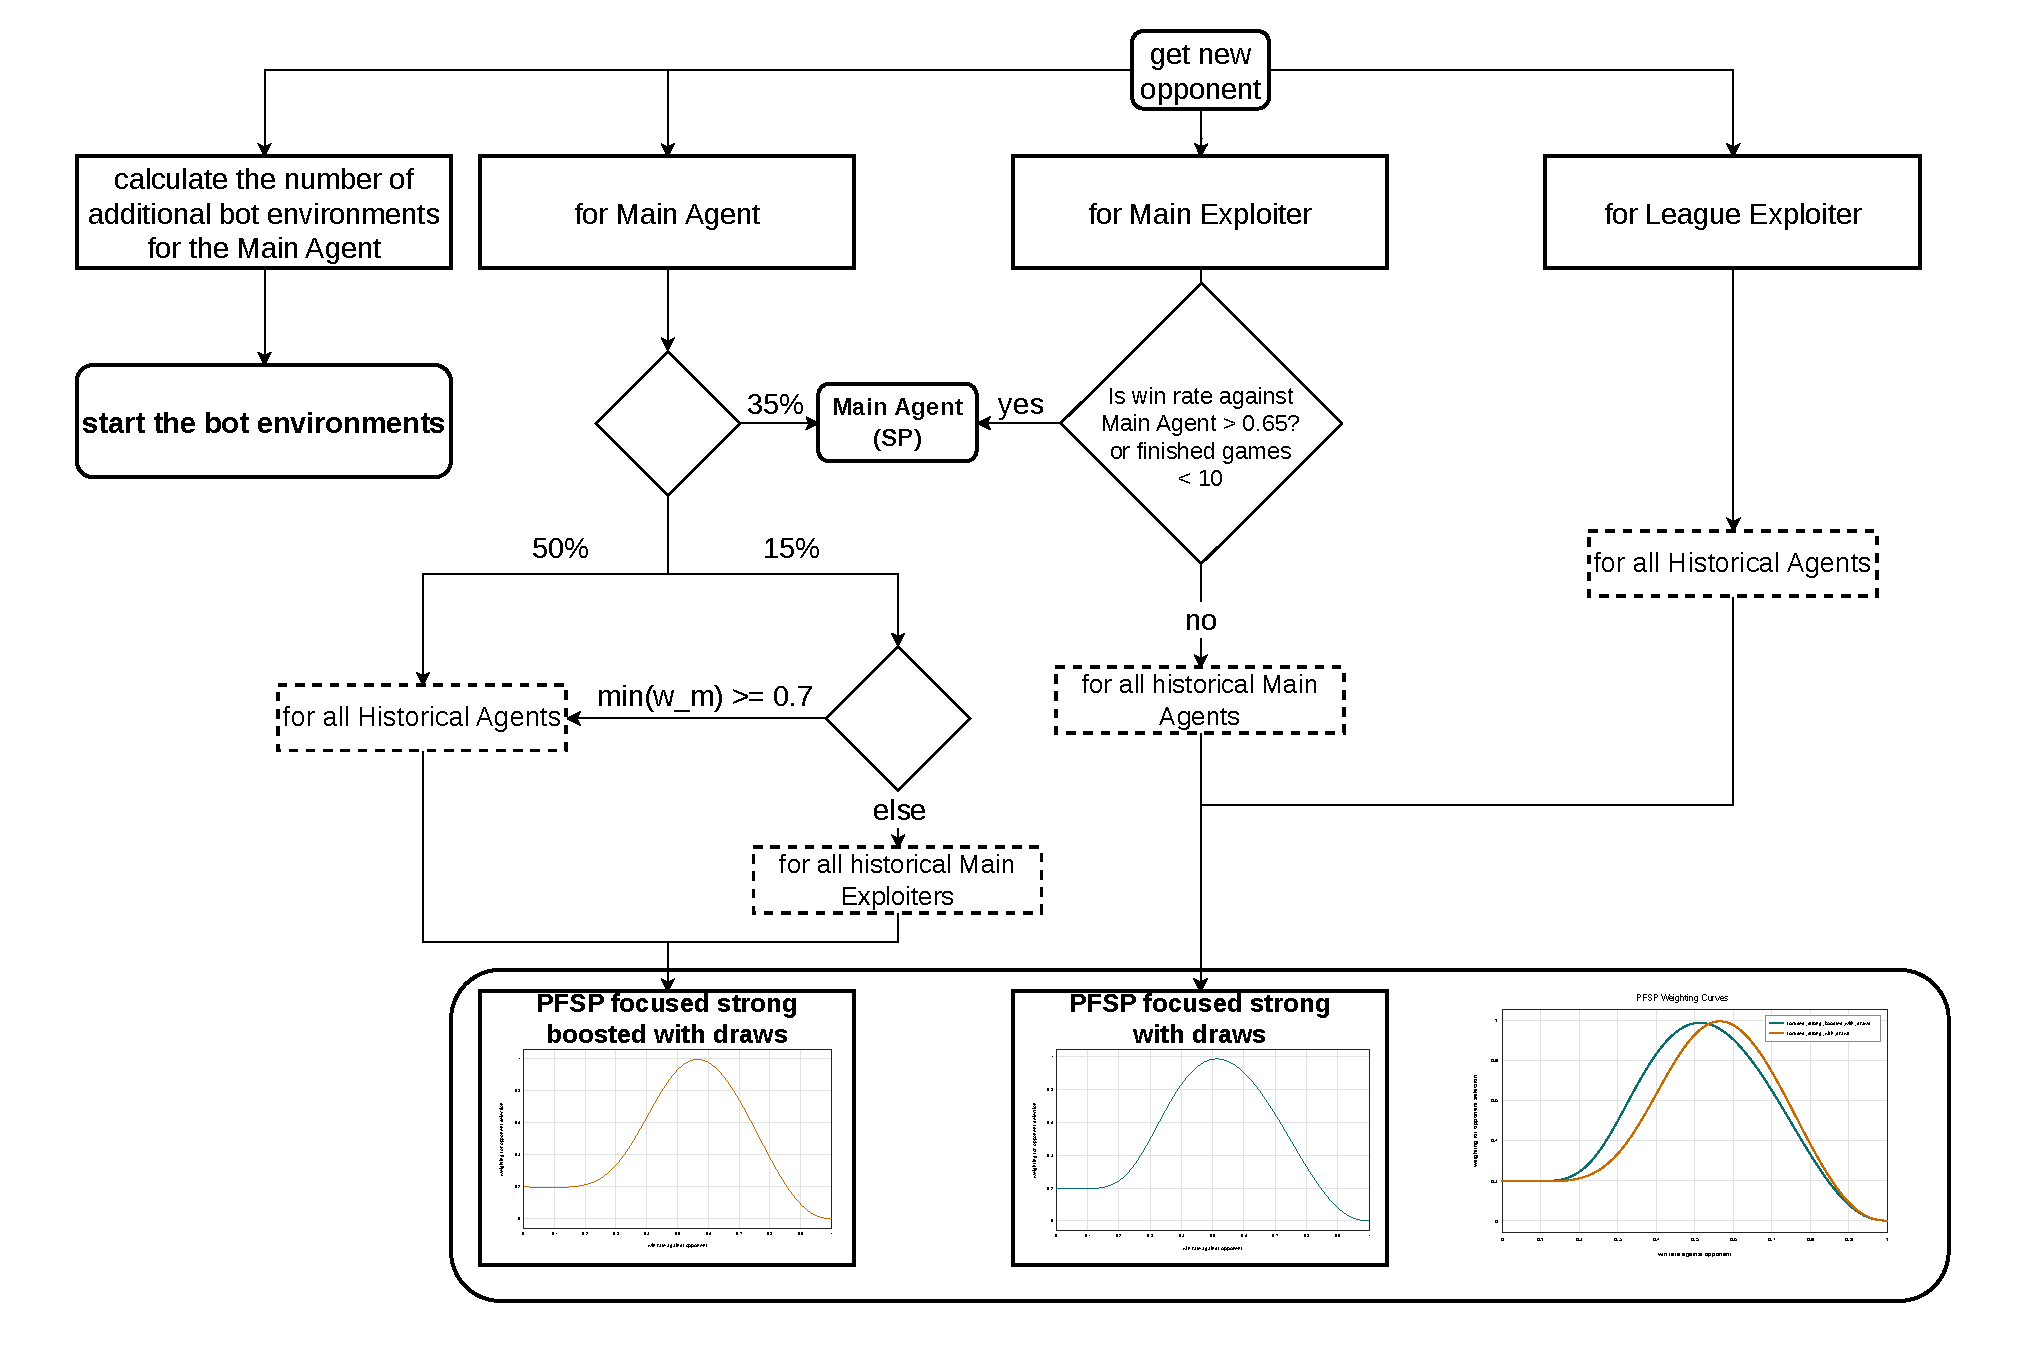
\includegraphics[width=\linewidth,height=0.80\textheight,keepaspectratio]{diagram_with_obs_presentation.pdf}
    \end{center}
    \vspace{-0.4em}
    \centering
    \scriptsize Matchmaking and opponent sampling in the LT setup.
\end{frame}



\begin{frame}[noframenumbering]{New Initial Agents}
    \small
    \centering
    \textbf{1 agent per unit type}\par
    \vspace{0.45em}

    {
    \renewcommand{\TrainingPipelineBoxHeight}{2.55cm}
    \begin{columns}[T,onlytextwidth]
        \begin{column}{0.49\textwidth}
            \TrainingPipelineCard{HHUBlue}{HHULight}{Heavy focused}{
                \begin{itemize}\setlength{\itemsep}{0.2em}
                    \item Base Agent
                \end{itemize}
            }
        \end{column}
        \begin{column}{0.49\textwidth}
            \TrainingPipelineCard{HHUBlue}{HHULight}{Light focused}{
                \begin{itemize}\setlength{\itemsep}{0.2em}
                    \item 9 epochs of BC with LightRushAI as the expert
                    \item opponents for BC: Mayari, WorkerRushAI, LightRushAI
                \end{itemize}
            }
        \end{column}
    \end{columns}

    \vspace{0.35em}

    \begin{columns}[T,onlytextwidth]
        \begin{column}{0.49\textwidth}
            \TrainingPipelineCard{HHUBlue}{HHULight}{Worker focused}{
                \begin{itemize}\setlength{\itemsep}{0.2em}
                    \item 8 epochs of BC with WorkerRushAI as the expert
                    \item opponents for BC: Mayari, WorkerRushAI, LightRushAI
                \end{itemize}
            }
        \end{column}
        \begin{column}{0.49\textwidth}
            \TrainingPipelineCard{HHUBlue}{HHULight}{Ranged focused}{
                \begin{itemize}\setlength{\itemsep}{0.2em}
                    \item 6 epochs of BC with CoacAI as the expert
                    \item 180 updates of PPO against the Base Agent, CoacAI and Mayari
                    \item opponents for BC: WorkerRushAI, LightRushAI, Mayari and CoacAI
                \end{itemize}
            }
        \end{column}
    \end{columns}
    }

\end{frame}


\begin{frame}[noframenumbering]{Why Not Fewer Environments?}
    \begin{itemize}
        \item The number of environments affects rollout size.
        \item Smaller rollouts make PPO updates more unstable because they provide less information about the update direction.
        \item More steps per rollout create similar tradeoffs to adding more environments.
    \end{itemize}
\end{frame}


\begin{frame}[noframenumbering]{win rates against Base Agent as player 2}
    \begin{itemize}
        \item P1: LT-FT against P2: Base Agent: win rate 85\%, draw rate 15\%, loss rate 0\%
        \item P2: LT-FT against P1: Base Agent: win rate 89\%, draw rate 11\%, loss rate 0\%
    \end{itemize}
\end{frame}


\end{document}
